% Options for packages loaded elsewhere
\PassOptionsToPackage{unicode}{hyperref}
\PassOptionsToPackage{hyphens}{url}
%
\documentclass[
  man]{apa7}
\usepackage{amsmath,amssymb}
\usepackage{iftex}
\ifPDFTeX
  \usepackage[T1]{fontenc}
  \usepackage[utf8]{inputenc}
  \usepackage{textcomp} % provide euro and other symbols
\else % if luatex or xetex
  \usepackage{unicode-math} % this also loads fontspec
  \defaultfontfeatures{Scale=MatchLowercase}
  \defaultfontfeatures[\rmfamily]{Ligatures=TeX,Scale=1}
\fi
\usepackage{lmodern}
\ifPDFTeX\else
  % xetex/luatex font selection
\fi
% Use upquote if available, for straight quotes in verbatim environments
\IfFileExists{upquote.sty}{\usepackage{upquote}}{}
\IfFileExists{microtype.sty}{% use microtype if available
  \usepackage[]{microtype}
  \UseMicrotypeSet[protrusion]{basicmath} % disable protrusion for tt fonts
}{}
\makeatletter
\@ifundefined{KOMAClassName}{% if non-KOMA class
  \IfFileExists{parskip.sty}{%
    \usepackage{parskip}
  }{% else
    \setlength{\parindent}{0pt}
    \setlength{\parskip}{6pt plus 2pt minus 1pt}}
}{% if KOMA class
  \KOMAoptions{parskip=half}}
\makeatother
\usepackage{xcolor}
\usepackage{graphicx}
\makeatletter
\def\maxwidth{\ifdim\Gin@nat@width>\linewidth\linewidth\else\Gin@nat@width\fi}
\def\maxheight{\ifdim\Gin@nat@height>\textheight\textheight\else\Gin@nat@height\fi}
\makeatother
% Scale images if necessary, so that they will not overflow the page
% margins by default, and it is still possible to overwrite the defaults
% using explicit options in \includegraphics[width, height, ...]{}
\setkeys{Gin}{width=\maxwidth,height=\maxheight,keepaspectratio}
% Set default figure placement to htbp
\makeatletter
\def\fps@figure{htbp}
\makeatother
\setlength{\emergencystretch}{3em} % prevent overfull lines
\providecommand{\tightlist}{%
  \setlength{\itemsep}{0pt}\setlength{\parskip}{0pt}}
\setcounter{secnumdepth}{-\maxdimen} % remove section numbering
% Make \paragraph and \subparagraph free-standing
\ifx\paragraph\undefined\else
  \let\oldparagraph\paragraph
  \renewcommand{\paragraph}[1]{\oldparagraph{#1}\mbox{}}
\fi
\ifx\subparagraph\undefined\else
  \let\oldsubparagraph\subparagraph
  \renewcommand{\subparagraph}[1]{\oldsubparagraph{#1}\mbox{}}
\fi
\newlength{\cslhangindent}
\setlength{\cslhangindent}{1.5em}
\newlength{\csllabelwidth}
\setlength{\csllabelwidth}{3em}
\newlength{\cslentryspacingunit} % times entry-spacing
\setlength{\cslentryspacingunit}{\parskip}
\newenvironment{CSLReferences}[2] % #1 hanging-ident, #2 entry spacing
 {% don't indent paragraphs
  \setlength{\parindent}{0pt}
  % turn on hanging indent if param 1 is 1
  \ifodd #1
  \let\oldpar\par
  \def\par{\hangindent=\cslhangindent\oldpar}
  \fi
  % set entry spacing
  \setlength{\parskip}{#2\cslentryspacingunit}
 }%
 {}
\usepackage{calc}
\newcommand{\CSLBlock}[1]{#1\hfill\break}
\newcommand{\CSLLeftMargin}[1]{\parbox[t]{\csllabelwidth}{#1}}
\newcommand{\CSLRightInline}[1]{\parbox[t]{\linewidth - \csllabelwidth}{#1}\break}
\newcommand{\CSLIndent}[1]{\hspace{\cslhangindent}#1}
\ifLuaTeX
\usepackage[bidi=basic]{babel}
\else
\usepackage[bidi=default]{babel}
\fi
\babelprovide[main,import]{english}
% get rid of language-specific shorthands (see #6817):
\let\LanguageShortHands\languageshorthands
\def\languageshorthands#1{}
% Manuscript styling
\usepackage{upgreek}
\captionsetup{font=singlespacing,justification=justified}

% Table formatting
\usepackage{longtable}
\usepackage{lscape}
% \usepackage[counterclockwise]{rotating}   % Landscape page setup for large tables
\usepackage{multirow}		% Table styling
\usepackage{tabularx}		% Control Column width
\usepackage[flushleft]{threeparttable}	% Allows for three part tables with a specified notes section
\usepackage{threeparttablex}            % Lets threeparttable work with longtable

% Create new environments so endfloat can handle them
% \newenvironment{ltable}
%   {\begin{landscape}\centering\begin{threeparttable}}
%   {\end{threeparttable}\end{landscape}}
\newenvironment{lltable}{\begin{landscape}\centering\begin{ThreePartTable}}{\end{ThreePartTable}\end{landscape}}

% Enables adjusting longtable caption width to table width
% Solution found at http://golatex.de/longtable-mit-caption-so-breit-wie-die-tabelle-t15767.html
\makeatletter
\newcommand\LastLTentrywidth{1em}
\newlength\longtablewidth
\setlength{\longtablewidth}{1in}
\newcommand{\getlongtablewidth}{\begingroup \ifcsname LT@\roman{LT@tables}\endcsname \global\longtablewidth=0pt \renewcommand{\LT@entry}[2]{\global\advance\longtablewidth by ##2\relax\gdef\LastLTentrywidth{##2}}\@nameuse{LT@\roman{LT@tables}} \fi \endgroup}

% \setlength{\parindent}{0.5in}
% \setlength{\parskip}{0pt plus 0pt minus 0pt}

% Overwrite redefinition of paragraph and subparagraph by the default LaTeX template
% See https://github.com/crsh/papaja/issues/292
\makeatletter
\renewcommand{\paragraph}{\@startsection{paragraph}{4}{\parindent}%
  {0\baselineskip \@plus 0.2ex \@minus 0.2ex}%
  {-1em}%
  {\normalfont\normalsize\bfseries\itshape\typesectitle}}

\renewcommand{\subparagraph}[1]{\@startsection{subparagraph}{5}{1em}%
  {0\baselineskip \@plus 0.2ex \@minus 0.2ex}%
  {-\z@\relax}%
  {\normalfont\normalsize\itshape\hspace{\parindent}{#1}\textit{\addperi}}{\relax}}
\makeatother

% \usepackage{etoolbox}
\makeatletter
\patchcmd{\HyOrg@maketitle}
  {\section{\normalfont\normalsize\abstractname}}
  {\section*{\normalfont\normalsize\abstractname}}
  {}{\typeout{Failed to patch abstract.}}
\patchcmd{\HyOrg@maketitle}
  {\section{\protect\normalfont{\@title}}}
  {\section*{\protect\normalfont{\@title}}}
  {}{\typeout{Failed to patch title.}}
\makeatother

\usepackage{xpatch}
\makeatletter
\xapptocmd\appendix
  {\xapptocmd\section
    {\addcontentsline{toc}{section}{\appendixname\ifoneappendix\else~\theappendix\fi\\: #1}}
    {}{\InnerPatchFailed}%
  }
{}{\PatchFailed}
\keywords{social feedback, socioeconomic status, area deprivation, negative affect, discrimination}
\DeclareDelayedFloatFlavor{ThreePartTable}{table}
\DeclareDelayedFloatFlavor{lltable}{table}
\DeclareDelayedFloatFlavor*{longtable}{table}
\makeatletter
\renewcommand{\efloat@iwrite}[1]{\immediate\expandafter\protected@write\csname efloat@post#1\endcsname{}}
\makeatother
\usepackage{csquotes}
\raggedbottom
\usepackage{helvet}
\renewcommand{\familydefault}{\sfdefault}
\ifLuaTeX
  \usepackage{selnolig}  % disable illegal ligatures
\fi
\IfFileExists{bookmark.sty}{\usepackage{bookmark}}{\usepackage{hyperref}}
\IfFileExists{xurl.sty}{\usepackage{xurl}}{} % add URL line breaks if available
\urlstyle{same}
\hypersetup{
  pdftitle={Socioeconomic status and adolescent brain responses to peer feedback: Testing the impact on negative affect},
  pdfauthor={Brent I. Rappaport1, James E. Glazer1, Lilian Y. Li1, Madeline M. McGregor1, Lili A. Massac2, Katherine Durham2, Randy P. Auerbach2, \& Stewart A. Shankman1},
  pdflang={en-EN},
  pdfkeywords={social feedback, socioeconomic status, area deprivation, negative affect, discrimination},
  hidelinks,
  pdfcreator={LaTeX via pandoc}}

\title{Socioeconomic status and adolescent brain responses to peer feedback: Testing the impact on negative affect}
\author{Brent I. Rappaport\textsuperscript{1}, James E. Glazer\textsuperscript{1}, Lilian Y. Li\textsuperscript{1}, Madeline M. McGregor\textsuperscript{1}, Lili A. Massac\textsuperscript{2}, Katherine Durham\textsuperscript{2}, Randy P. Auerbach\textsuperscript{2}, \& Stewart A. Shankman\textsuperscript{1}}
\date{}


\shorttitle{SES \& peer feedback}

\authornote{

The authors made the following contributions. Brent I. Rappaport: Conceptualization, Formal analysis, Writing - Original Draft Preparation, Writing - Review \& Editing; James E. Glazer: Methodology, Writing - Review \& Editing; Lilian Y. Li: Methodology, Writing - Review \& Editing; Madeline M. McGregor: Writing - Review \& Editing; Lili A. Massac: Writing - Review \& Editing; Katherine Durham: Writing - Review \& Editing; Randy P. Auerbach: Conceptualization, Fundind acquisition, Investigation, Methodology, Resources, Supervision, Writing - Review \& Editing; Stewart A. Shankman: Conceptualization, Fundind acquisition, Investigation, Methodology, Resources, Supervision, Writing - Review \& Editing.

Correspondence concerning this article should be addressed to Brent I. Rappaport, 680 N. Lakeshore Drive, Suite 1520, Chicago, IL 60611. E-mail: \href{mailto:brent.rappaport@northwestern.edu}{\nolinkurl{brent.rappaport@northwestern.edu}}

}

\affiliation{\vspace{0.5cm}\textsuperscript{1} Department of Psychiatry, Feinberg School of Medicine, Northwestern University\\\textsuperscript{2} Columbia University}

\abstract{%
Lower socioeconomic status (SES) is a potent risk factor for psychopathology in youth, however the mechanisms linking them are yet unknown. One potential neural mechanism is aberrant brain responding to peer acceptance and rejection. Objective: Test whether SES (operationalized as area deprivation) is 1) related to brain responses to peer feedback, and 2) moderates the relationship between brain responses to peer feedback and affect. Methods: 159 adolescent participants (ages 13-19) from the Chicago, IL and New York, NY metro areas completed an event-related potential (ERP) version of the Chatroom task, a week of ecological momentary assessment (EMA) reporting on their positive and negative affect, and a self-report of discrimination (adolescent discrimination distress index). Results: lower SES (as well as greater self-reported discrimination distress) was related to blunted responses to acceptance. Moreover, brain responses to rejection interacted with SES to predict EMA reported negative, but not positive, affect. Conclusion: SES may be linked to depression and anxiety disorders via heightened sensitivity to rejection, and/or blunted responses acceptance. Preliminary evidence suggests that discrimination may be one factor of low SES driving this effect. This study uses multiple levels of analysis (objective measure of environment, brain activity, EMA reported affect) to identify a potential brain x environment mechanisms explaining why low SES are at higher risk for internalizing disorders.
}



\begin{document}
\maketitle

\newpage{}

Low socioeconomic status (SES) in youth is a robust correlate of concurrent psychopathology (McLaughlin et al., 2012; Peverill et al., 2021a) and longitudinal predictor of psychopathology and general health problems into adulthood (Ferraro et al., 2016; Santiago et al., 2011). However, the mechanisms linking SES to psychopathology remain unknown. This study examines whether one potential mechanism interacts with this sociological stressor to influence individual mental health: anomalous processing of feedback from others. That is, does a greater sensitivity to rejection and/or blunted sensitivity to acceptance from others, in combination with low SES, produce worse mental health outcomes.

Lower SES youth experience greater prejudice, discrimination, and stigma from others than higher SES youth (Cozzarelli et al., 2001; Moura et al., 2019) leading to biases in how they interpret social situations. Numerous theories (Crick \& Dodge, 1994; Simons et al., 2012) have argued that discrimination, prejudice, and stigma leads to difficulty being open, trusting and intimate with others (Rokach \& Clayton, 2023), along with other social biases. Chronic discriminatory experiences lead to distrustful, cynical relationship schemas (Simons et al., 2012; Simons \& Burt, 2011); that is, longstanding beliefs, cognitions, and expectations about social relationships (Baldwin, 1995). Youth develop these relationship schemas from experience with others. These schemas, in turn, help youth to efficiently identify salient social information (Crick \& Dodge, 1994). Thus, when youth regularly experience discrimination, the schema adapts to expect it in social interactions. Two ways this can manifest in social interactions are: 1) heightened sensitivity to negative feedback (rejection), and 2) blunted sensitivity to positive feedback (acceptance). These biases can have short-term benefits such as leading the individual to safely remove themselves from hostile environments (Allen \& Badcock, 2003; Gilbert, 2006). Over time, however, chronic heightened rejection sensitivity and blunted acceptance sensitivity can lead to pervasive social withdrawal and depressive and anxiety disorders (Ike et al., 2020).

Chronic heightened rejection sensitivity and blunted acceptance sensitivity have been tied to internalizing disorders. Enhanced sensitivity to rejection is related to depression (Eisenberger et al., 2009; Groschwitz et al., 2016; Harms et al., 2019; Jankowski et al., 2018; Kumar et al., 2017; Pegg et al., 2021) and socially relevant anxiety (i.e., behavioral inhibition, social anxiety disorder, generalized anxiety) in youth (Beer et al., 2016; Guyer et al., 2014; Rappaport \& Barch, 2020). Likewise, blunted sensitivity to acceptance is also related to depression (Kujawa et al., 2017; Olino et al., 2015; Pegg et al., 2021; Zhang et al., 2017). Such brain patterns can result in functional impairments: fearing social situations or not finding them pleasurable, youth withdraw hampering their ability to form and maintain positive peer relationships. This is a particularly important aspect of healthy adolescent development. Therefore, understanding how low SES confers risk for psychopathology may lead to reduced clinical symptoms and improved functioning.

\hypertarget{current-study}{%
\subsection{Current Study}\label{current-study}}

Despite prior studies showing links between SES and psychopathology (e.g., McLaughlin et al., 2012; Peverill et al., 2021b) and brain responses to peer feedback and psychopathology (e.g., Guyer et al., 2014; Kujawa et al., 2017; Pagliaccio et al., 2022; Rappaport \& Barch, 2020), there is only one study showing a link between SES and brain responses to peer feedback (Rappaport et al., 2023). The current study aims to fill this gap by explicitly testing whether an objective and validated measure of SES (area deprivation index {[}ADI; Kind et al., 2014; Kind \& Buckingham, 2018; Knighton et al., 2016{]}) is related to brain responses to peer feedback and moderates the association between these brain responses and negative affect in adolescents.

The first aim of the study tests whether low SES relates to brain responses to different kinds of peer feedback (acceptance and rejection). To measure brain responses to peer feedback, this study used event-related potentials (ERPs)---fluctuations in electroencephalography (EEG) signals that are time-locked to particular events. Unlike other neural measures like fMRI, ERPs have high temporal resolution (on the order of milliseconds) making them ideal for detecting separate neuropsychological responses to peer feedback. For example, the reward positivity (RewP)---a positive inflection that occurs around 250-350ms post feedback and is maximal at frontocentral cites (Proudfit, 2015)---likely reflects the rewarding aspects of acceptance in peer feedback studies (Ethridge et al., 2017; Funkhouser et al., 2020). Alternatively, the P3---a positive inflection occurring around 300ms post feedback and maximal at centroparietal sites---likely reflects the salient aspects of acceptance and rejection in peer feedback studies (Funkhouser et al., 2020; Pegg et al., 2022). This makes ERP ideal for testing whether low SES is related to a) more blunted sensitivity to acceptance in the RewP, b) heightened salience of rejection in the P3, or c) both.

The second aim of the study was to test whether SES moderates the relationship between brain responses to peer feedback and negative affect assessed via ecological momentary assessment (EMA). Unlike traditional self-report assessments, EMA provides ecologically valid indicators of affect outside of the lab, as adolescents go about their daily lives. Furthermore, as EMA collects multiple samples of affect per participant, it yields more accurate measures of mean affect than single snapshot assessments and is less susceptible to biases associated with retrospective recall (Moskowitz \& Young, 2006; Solhan et al., 2009). Critically, showing that SES moderates the relationship between brain responses to peer feedback and negative affect would support heightened neural rejection sensitivity and/or blunted acceptance sensitivity as potential clinical targets for prevention/intervention. For example, targeted interventions aimed at reducing rejection sensitivity could reduce low SES youths' risk for later life psychopathology.

The third aim of this study was to test the above two aims with a critical correlate of low SES---perceived discrimination. Low SES youth often experience greater discrimination, either directly due to their economic standing or due to other conflated factors\footnote{Due to sociological factors including systemic oppression of racial minorities, racial minority youth tend to be poorer and also more discriminated against than racial majority youth (Drake \& Rank, 2009; Thompson \& Suarez, 2019).} (Cozzarelli et al., 2001; Moura et al., 2019; Williams, 1999). Perceived discrimination, specifically, has been linked to greater negative affect (Deckard et al., 2023). However, no study has tested whether perceived discrimination is related to altered patterns of brain responses to peer feedback. This aim also complements the above aims with SES as it examines a subjective correlate (Watson et al., 2002), and more specific aspect, of SES. That is, while SES is a broad construct, perceived discrimination is a more specific consequence of low SES that may be particularly relevant to adolescent brain responses to peer feedback and subsequent risk for psychopathology. Indeed, perceived discrimination is as strong a risk factor for psychopathology as other significant life events (e.g., loss of a loved one or job loss), and comparable risk factor for depression and anxiety to traumatic events (e.g., sexual assault and combat; Kessler et al., 1999).

\hypertarget{methods}{%
\section{Methods}\label{methods}}

\hypertarget{participants}{%
\subsection{Participants}\label{participants}}

Participant data was acquired from a larger, ongoing project examining social processing deficits in adolescent depression. Adolescents, ages 13-18-years-old, were recruited from the community (via ads on public transportation, Facebook, and craigslist) and mental health clinics in New York City, NY and Chicago, IL. Informed assent and consent were obtained from the adolescent and parent, respectively, and adolescents 18 years or older provided consent. All study procedures were carried out in accordance with the Declaration of Helsinki and approved by the New York State Psychiatric (NYSPI) (primary) Institutional Review Board (IRB) and the Northwestern University IRB. General inclusion criteria included: (a) Tanner Stage \(\ge\) 3 (Tanner \& Davies, 1985), (b) parental and child fluency in English, (c) Wechsler Abbreviated Scale of Intelligence-II (WASI-II) \textgreater{} 85 (Wechsler, 2011), (d) ownership of a personal smartphone (android or iOS), and (e) right-handedness. General exclusion criteria included: (a) history of head injury or neurologicaldf disorders, (b) current moderate or severe substance use disorder, and (c) lifetime history of bipolar or psychotic disorders, oppositional defiant disorder, conduct disorder, organic mental disorder, or developmental disorder. N=160 participants were available to analyze for the present study. Table 1 summarizes the participant demographic and clinical characteristics.

\begin{table}[tbp]

\begin{center}
\begin{threeparttable}

\caption{\label{tab:demoTable}}

\begin{tabular}{llllll}
\toprule
Variable & \multicolumn{1}{c}{Columbia (N=90)} & \multicolumn{1}{c}{Northwestern (N=70)} & \multicolumn{1}{c}{p} & \multicolumn{1}{c}{sig} & \multicolumn{1}{c}{es}\\
\midrule
Age & 16.63 (1.49) & 16.44 (1.55) & .44 &  & d=-0.12\\
SES & 83.51 (18.06) & 70.19 (16.95) & <.001 & *** & d=-0.76\\
Sex (Male) & 23 (25.56\%) & 22 (32.35\%) & .45 &  & OR=1.39\\
Hispanic ethnicity (Yes) & 33 (36.67\%) & 21 (30.43\%) & .51 &  & OR=0.76\\
demo\_child\_race & - & - & .10 &  & V=0.11\\
American Indian/Alaska Native & 1 (1.11\%) & 1 (1.45\%) & - & - & -\\
Asian & 18 (20\%) & 9 (13.04\%) & - & - & -\\
Black or African American & 7 (7.78\%) & 7 (10.14\%) & - & - & -\\
More than one race & 14 (15.56\%) & 5 (7.25\%) & - & - & -\\
Native Hawaiian or Other Pacific Islander & 1 (1.11\%) & - & - & - & -\\
Unknown or not reported & 14 (15.56\%) & 5 (7.25\%) & - & - & -\\
White & 35 (38.89\%) & 42 (60.87\%) & - & - & -\\
IDAS depression & 2.22 (0.92) & 1.86 (0.79) & .010 & ** & d=-0.42\\
Lifetime number of stressors & 29.02 (14.53) & 20.97 (14.04) & <.001 & *** & d=-0.56\\
Lifetime stressor severity & 68.55 (39.44) & 46.9 (35.01) & <.001 & *** & d=-0.58\\
\bottomrule
\addlinespace
\end{tabular}

\begin{tablenotes}[para]
\normalsize{\textit{Note.} Note. N=1 excluded for missing group variable. N=3 missing Age. N=1 missing SES. N=2 missing Sex. N=1 missing Hispanic ethnicity. N=1 missing Race. N=3 missing IDAS depression. N=3 missing Lifetime number of stressors. N=3 missing Lifetime stressor severity. * p<.05, ** p<.01, *** p<.001}
\end{tablenotes}

\end{threeparttable}
\end{center}

\end{table}

\hypertarget{procedure}{%
\subsection{Procedure}\label{procedure}}

\hypertarget{chatroom-task}{%
\subsubsection{Chatroom task}\label{chatroom-task}}

The Chatroom Task (Guyer et al., 2008, 2009) was completed over two visits. At consent, participants were told that they were participating in a multi-site study on adolescent interactions in online chat rooms. Participants created profiles including their likes/dislikes and a photograph taken in the lab; they were told that other participants would review their profile and indicate interest (acceptance) or not (rejection) in chatting. Next, participants viewed photographs of 100 same-sex peers and selected 50 that they were `interested' (high value) and 50 that they were `not interested' (low value) in chatting with online following the EEG task. On each of 100 trials during EEG recording (\textasciitilde1 week later; Figure 1), a peer photograph was displayed with a reminder of participants' prior choice: `You were {[}not{]} interested', followed by a fixation cross for a jittered inter-stimulus interval. Next, peer acceptance or rejection feedback was displayed: `Interested' or `Not Interested' (feedback type), followed by a second jittered ISI. Finally, participants rated their emotional response (rating). Participants received 50 acceptance and 50 rejection trials (split by participant interest, e.g., n = 25 when participants were interested and accepted), pseudorandomized with no more than three sequential acceptances/rejections. After EEG recording was completed, we assessed whether participants believed that they would be able to chat with the peers after the task (``While you were doing the chatroom, did you believe that you would really be chatting with one of these people on the computer after your EEG?'' ), as well as ``why not'' if they endorsed not believing that they would be able to chat with them. Finally, participants were debriefed on the deception.

Importantly, the structure of the task results in four within-subject conditions: 1) acceptance from high-value peers (i.e., peers that participants were interested in talking to), 2) rejection from high-value peers, 3) acceptance from low-value peers (i.e., peers that participants were not interested in talking to), and 4) rejection from low-value peers.

\hypertarget{eeg-recording-and-processing}{%
\subsubsection{EEG recording and processing}\label{eeg-recording-and-processing}}

Continuous EEG data were recorded during the Chatroom task using the 32-channel ActiCHamp from Brain Products (Brain Products, Munich, Germany), digitized at a 500 Hz sampling rate, and referenced online to FCz. Vertical and horizontal EOG data were recorded, and electrode impedances were maintained below 20 K\(\Omega\). EEG data were processed offline using EEGLAB version 2022.1 (Delorme \& Makeig, 2004) and ERPLAB version 9.00 (Lopez-Calderon \& Luck, 2014) toolboxes in MATLAB version r2022b. Independent component analysis (ICA) and automated identification (ICLabel version 1.4) was used to identify and correct for ocular artifacts prior to artifact rejection. Data were re-referenced offline using an average mastoid reference. A notch filter (60 Hz) and a second-order digital Butterworth filter with a bandpass from 0.1 to 30 Hz were applied. Trials were epoched from -200 to 2000ms and baseline-adjusted by subtracting the average amplitude for 200 ms prior to the stimulus onset (-200 to 0ms).

Stimulus-locked ERPs were averaged separately for each combination of peer value (high, low) and feedback type (acceptance, rejection). Grand averages were inspected to determine time windows to be extracted (see Figure 1). Time windows were chosen based on those time windows which showed substantial difference between condition, and which are consistent with prior literature (Donaldson et al., 2016; Funkhouser et al., 2020; Pegg et al., 2022) for the N1, a time window of 50-150ms was used, for the RewP: 150-275ms, and for the P3: 275-425ms. Mean amplitude within each time window was computed at Cz electrode. Because this is the first study to examine ERP components of the Chatroom task, we sought to use the same electrode for all ERP components for consistency. twelve subjects were excluded for too few clean trials following artifact rejection. This resulted in a sample of N= 172 with clean N1 data, 159 with clean RewP data, and N= 161 with clean P300 data.

\begin{figure}
\centering
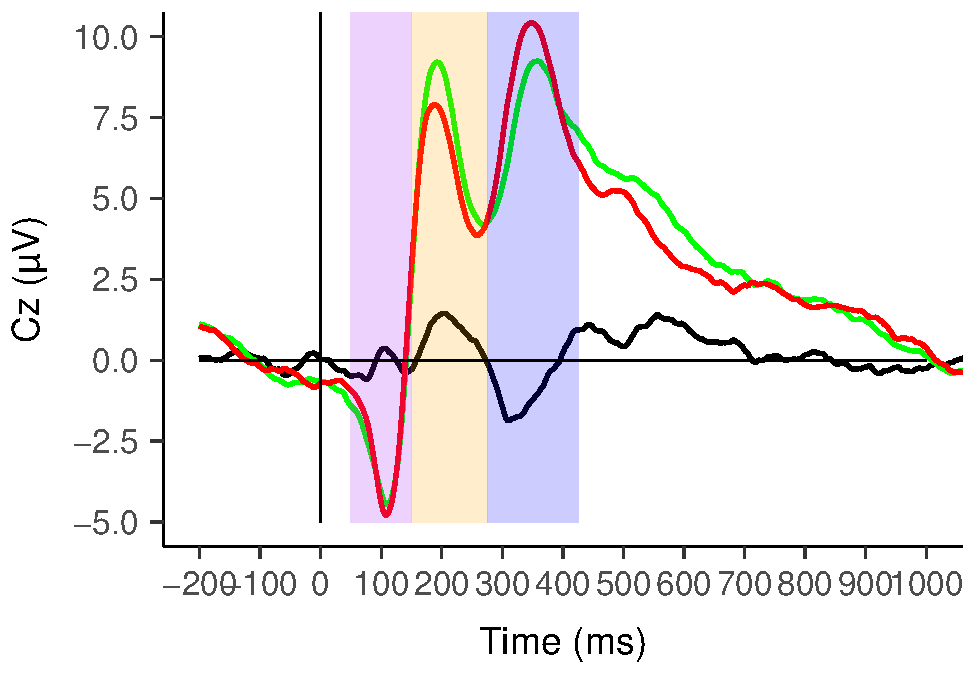
\includegraphics{BUDS_manuscript_working_files/figure-latex/grandAverage-1.pdf}
\caption{\label{fig:grandAverage}Grand average ERP for acceptance and rejection feedback from high-value peers. Colored sections of the graph represent time windows where ERP components were extracted at Cz electrode: N1 = purple, RewP = orange, P300 = blue}
\end{figure}

\hypertarget{ecological-momentary-assessment-ema}{%
\subsubsection{Ecological momentary assessment (EMA)}\label{ecological-momentary-assessment-ema}}

Ecological momentary assessment data was collected using the Effortless Assessment of Risk States (EARS) app (Lind et al., 2018; Lind et al., 2023). For seven days after consenting into the study, participants received three notifications each day prompting them to complete a set of 11-items regarding their current mood and social interactions. These notifications were sent between 6:30am-8:30am, 3:00pm-5:00pm, and 7:00-10:00pm. Surveys were available for 90 minutes after the initial notification and participants were able to decline answering any question. Participants were compensated 1 dollar for every completed set of questions for a maximum of 3 dollars per day and 21 dollars total. Participants rated 11 items on a scale from 0 (\emph{not at all})-100 (\emph{extremely}). They rated how happy, excited, supported, angry, anxious, sad, and rejected they felt. The first three were averaged into a positive affect composite, and the latter four in a negative affect composite. For both composites, listwise deletion was used (i.e., if subjects were missing a value for ``sad'' their negative affect composite score was missing for that time point.

\hypertarget{measures}{%
\subsection{Measures}\label{measures}}

\hypertarget{ses-area-deprivation-index-adi}{%
\subsubsection{SES: Area Deprivation Index (ADI)}\label{ses-area-deprivation-index-adi}}

The area deprivation index (Kind \& Buckingham, 2018; University of Wisconsin School of Medicine and Public Health, 2023) is a composite measure based on 17 dimensions of socioeconomic disadvantage including education, employment, housing quality, and poverty-related factors, all measured via the American Community Survey. Neighborhoods are determined based on census tracts and are assigned a percentile from 1 to 100, where a higher percentile indicates greater levels of neighborhood disadvantage. In cases when ADI values were missing for subjects (e.g., suppression due to a high group quarter population), it was estimated using the ADI of the nearest census tract with available data. This was often tracts \textless1 mile from the original address. Of note, we reverse scored ADI percentile to create a more interpretable measure of SES (i.e., higher scores represent greater SES/lower ADI).

\hypertarget{discrimination-distress-adolescent-discrimination-distress-index-addi}{%
\subsubsection{Discrimination distress: Adolescent Discrimination Distress Index (ADDI)}\label{discrimination-distress-adolescent-discrimination-distress-index-addi}}

Discrimination-related distress was measured using the Adolescent Discrimination Distress Index (ADDI, Fisher et al., 2000). The ADDI is a 15-item self-report measure that assesses the distress experienced in response to perceived racial-ethnic discrimination across institutional, educational, and peer contexts. Each item includes a statement outlining a common example of discrimination (i.e.~``You were called racially insulting names''; ``You were wrongly disciplined or given after-school detention''). If a participant endorses that they experienced a given sample of discrimination on account of their race or ethnicity, they are then asked to rate how much the experience upset them on a five-point Likert scale from ``not at all'' to ``extremely''. In the current study, full-scale summary scores were used, where higher scores indicate greater discrimination-related distress. Given the format of ADDI, which requires participants to endorse whether an experience occurred in order to report its severity, Cronbach's alpha could not be measured.

\hypertarget{covariates}{%
\subsubsection{Covariates}\label{covariates}}

\hypertarget{depression-and-anxiety-symptoms-inventory-of-depression-and-anxiety-symptoms-idas-ii}{%
\paragraph{Depression and anxiety symptoms: Inventory of depression and anxiety symptoms (IDAS-II)}\label{depression-and-anxiety-symptoms-inventory-of-depression-and-anxiety-symptoms-idas-ii}}

The expanded Inventory of Depression and Anxiety Symptoms (IDAS-II; Watson, et al., 2012) is a 99-item, self-report instrument that measures the severity of depression, anxiety, and bipolar disorder symptoms over the past two weeks. Items are scored on a 5-point scale (1 = not at all; 5 = extremely). For the present study, 52-items were selected to assess current depression and anxiety symptoms. The depression and anxiety (a combination of the panic and social anxiety subscales) both demonstrated excellent internal consistency (Cronbach's alpha = 0.94, 0.90).

\hypertarget{stressful-life-events-and-severity-of-stressful-life-events-stress-and-adversity-inventory-strain}{%
\paragraph{Stressful life events and severity of stressful life events: Stress and adversity inventory (STRAIN)}\label{stressful-life-events-and-severity-of-stressful-life-events-stress-and-adversity-inventory-strain}}

The Stress and Adversity Inventory for Adolescents (STRAIN, Slavich et al., 2019) was administered to measure participants' exposure to acute and lifetime stressors. This interview assesses exposures to 75 different stressors across 12 primary life domains (i.e.~Housing, Education, Work, Treatment/Health, Marital/Partner, Reproduction, Financial, Legal/Crime, Other Relationships, Parent/Guardian, Death, Life-Threatening Situations) and five social-psychological characteristics (i.e.~Interpersonal Loss, Physical Danger, Humiliation, Entrapment, Role Change/Disruption). If a participant endorses a stressor, they are then asked additional questions about its severity, frequency, timing, and duration. Based on these answers, the STRAIN produces a summary score that notes participants' total lifetime stressor count and severity for all the acute life events and chronic difficulties experienced. Here, higher scores indicate greater stress exposure. In prior studies, the STRAIN has shown excellent test-retest reliability for total lifetime stressor count and severity over 2-4 weeks (\(r\) = 0.90---0.95, Cazassa et al., 2020; Slavich \& Shields, 2018). Given the format of the STRAIN, which requires participants to endorse whether a stressor occurred in order to report its severity, Cronbach's alpha could not be measured.

\hypertarget{data-analysis}{%
\subsection{Data analysis}\label{data-analysis}}

\hypertarget{behavioral-ratings}{%
\subsubsection{Behavioral ratings}\label{behavioral-ratings}}

Omnibus ANOVAs also tested whether in-task behavioral ratings varied as a function of Peer value (high, low) and Feedback type (acceptance and rejection). Post-hoc paired samples t-tests were used to compare levels of Peer value and Feedback type.

\hypertarget{erp-task-effects}{%
\subsubsection{ERP task effects}\label{erp-task-effects}}

Omnibus MLMs tested whether mean ERP amplitude varied as a function of Peer value (high, low) and Feedback type (acceptance and rejection). These models included random intercept effects of a) subject and b) study site.

\hypertarget{multilevel-multiple-regression-models}{%
\subsubsection{Multilevel multiple regression models}\label{multilevel-multiple-regression-models}}

\hypertarget{ses-related-to-erp-residualized-scores}{%
\paragraph{SES related to ERP residualized scores}\label{ses-related-to-erp-residualized-scores}}

For aim 1, we tested whether residualized scores (e.g., RewP\textsubscript{resid}) were associated with SES. This was examined for residualized scores to acceptance and rejection for each component (N1\textsubscript{resid}, RewP\textsubscript{resid}, P300\textsubscript{resid}).

\hypertarget{ses-moderating-association-between-erp-and-ema-measures-of-affect}{%
\paragraph{SES moderating association between ERP and EMA measures of affect}\label{ses-moderating-association-between-erp-and-ema-measures-of-affect}}

For aim 2, multilevel multiple regression models (MLMs) tested whether ERP amplitudes moderated associations between SES and negative affect. These models included random intercept effects of subject and study site. This assured that models predicted each subject's mean-level negative affect over the week. In some models, the random effect of site accounted for so little variance (likely due to the fact that there were only two sites) that the model was singular (i.e., that the variance of the random effect was essentially zero); in these cases site was included instead as a fixed effect (i.e., covariate). Given a positive skew and large number of 0's in the measure of negative affect, negative affect was cube-root transformed and zero-inflated Gaussian multilevel models were used. Visual diagnostic checks for model assumptions were conducted to assure that models were accurately specified (e.g., posterior predictive checks, homogeneity of variance, normality of residuals, colinearity, and normality of random effects). All predictors were included in both the condition and zero-inflation portions of the model.

\hypertarget{results}{%
\section{Results}\label{results}}

\hypertarget{behavioral-ratings-to-peer-feedback}{%
\subsection{Behavioral ratings to peer feedback}\label{behavioral-ratings-to-peer-feedback}}

\hypertarget{in-task-ratings}{%
\subsubsection{In-task ratings}\label{in-task-ratings}}

\begin{figure}
\centering
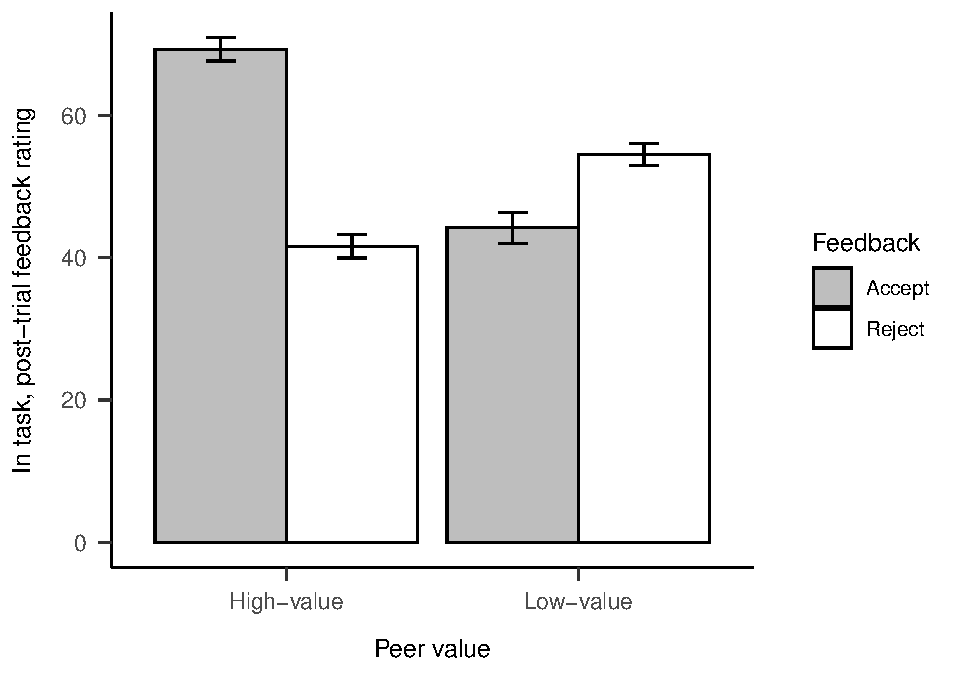
\includegraphics{BUDS_manuscript_working_files/figure-latex/rating_plot-1.pdf}
\caption{(\#fig:rating\_plot)Mean ratings across all participants by Feedback and Value.}
\end{figure}

Participants rated how they felt in each trial, immediately after receiving feedback, on a scale from 0 (``Very angry'') to 100 (``Very good''). Omnibus MLMs showed a significant Peer value x Feedback type interaction (\(b = -37.54\), 95\% CI \([-41.06, -34.01]\), \(t(655) = -20.92\), \(p < .001\)), such that participants rated acceptance from high-value peers (i.e., peers that they were interested in) as feeling significantly better than rejection from high-value peers (\(M_D = 27.63\), 95\% CI \([24.87, 30.40]\), \(t(165) = 19.73\), \(p < .001\)). However, participants rated feeling more angry in response to acceptance than rejection from low-value peers (\(M_D = -10.25\), 95\% CI \([-13.29, -7.21]\), \(t(165) = -6.65\), \(p < .001\)).\footnote{This somewhat surprising/counterintuitive finding is discussed further in the Discussion.}

\hypertarget{post-task-ratings}{%
\subsubsection{Post-task ratings}\label{post-task-ratings}}

To assess whether participants were deceived by the task, during post-task debriefing, 129 participants responded `yes' and 27 participants responded `no' to the question ``While you were doing the chatroom, did you believe that you would really be chatting with one of these people on the computer after your EEG?'' (N= 3 were missing debriefing data). Given the potential for deception to affect results, we present additional analyses covarying for this in the Supplement.

\hypertarget{brain-responses-to-peer-feedback}{%
\subsection{Brain responses to peer feedback}\label{brain-responses-to-peer-feedback}}

\hypertarget{task-effects-feedback-x-value-interaction}{%
\subsubsection{Task effects: Feedback x Value interaction}\label{task-effects-feedback-x-value-interaction}}

Omnibus MLMs showed that Peer value interacted with Feedback type to predict ERP mean amplitude for ERP components consistent with an N1 (\(\hat{\beta} = -0.79\), 95\% CI \([-1.49, -0.10]\), \(t(510.00) = -2.24\), \(p = .026\)), RewP (\(\hat{\beta} = -2.92\), 95\% CI \([-3.88, -1.95]\), \(t(471) = -5.92\), \(p < .001\))\footnote{Included site as a fixed effect covariate because models including it as a random effect resulted in singular fit.} and P300 (\(\hat{\beta} = -2.18\), 95\% CI \([-3.36, -0.99]\), \(t(477) = -3.59\), \(p < .001\)). These ERP components had time courses and scalp topographies (central around Cz electrode) consistent with an N1 (50-150ms), reward positivity (RewP; 150-275ms) and P300 (275-425ms). Follow-up analyses showed that the N1 (\(M_D = 0.64\), 95\% CI \([0.14, 1.14]\), \(t(171) = 2.52\), \(p = .013\)), RewP (\(M_D = 3.79\), 95\% CI \([3.04, 4.53]\), \(t(158) = 10.03\), \(p < .001\)), and P300 (\(M_D = 1.72\), 95\% CI \([0.89, 2.55]\), \(t(160) = 4.11\), \(p < .001\)) differentiated between acceptance and rejection for low-value peers. Only the RewP (\(M_D = 0.80\), 95\% CI \([0.24, 1.37]\), \(t(158) = 2.81\), \(p = .006\)) differentiated between acceptance and rejection for high-value peers, but not the N1 (\(M_D = -0.47\), 95\% CI \([-1.27, 0.32]\), \(t(160) = -1.17\), \(p = .243\)), nor P300 (\(M_D = -0.47\), 95\% CI \([-1.27, 0.32]\), \(t(160) = -1.17\), \(p = .243\)).

\hypertarget{internal-consistency}{%
\subsubsection{Internal consistency}\label{internal-consistency}}

The RewP and P300 demonstrated acceptable levels of internal consistency across peer-value (high, low) and feedback conditions (acceptance, rejection), with split-half reliability \textgreater{} 0.73, with particularly high reliability for the high-value peers conditions (acceptance and rejection r = 0.82 and 0.82 and 0.84 and 0.83; see Supplement). The N1 did not achieve acceptable internal consistency (r = 0.35-0.54).

\hypertarget{dependability}{%
\subsubsection{Dependability}\label{dependability}}

In dependability analyses, the ERPs to acceptance and rejection at the Cz electrode from 150-275ms and 275-425ms achieved acceptable dependability (\(\ge\) 0.70) with as few as 12-13 trials and the P300 with as few as 11-13 trials, depending on the peer-value and feedback condition. When using all available trials--up to 25 trials per condition--,they also achieved good dependability (\(\ge\) 0.80; see Supplement). ERPs to acceptance and rejection at the Cz electrode from 50-150ms did not achieve acceptable dependability with any number of trials (as many as 25 per condition).

\hypertarget{ses}{%
\subsubsection{SES}\label{ses}}

\hypertarget{ses-associations-with-n1resid-rewpresid-and-p300resid}{%
\paragraph{\texorpdfstring{SES associations with N1\textsubscript{resid}, RewP\textsubscript{resid}, and P300\textsubscript{resid}}{SES associations with N1resid, RewPresid, and P300resid}}\label{ses-associations-with-n1resid-rewpresid-and-p300resid}}

\begin{figure}
\centering
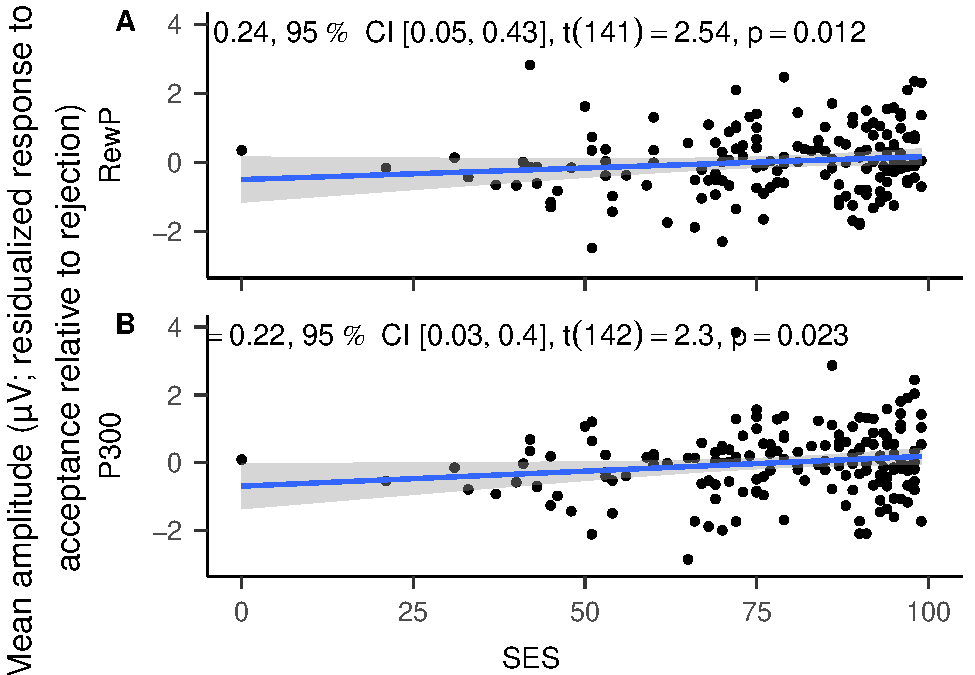
\includegraphics{BUDS_manuscript_working_files/figure-latex/adi_erp-1.pdf}
\caption{(\#fig:adi\_erp)Relationship between SES and brain responses to acceptance (relative to rejection) for both the RewP and P300 ERP components.}
\end{figure}

We found support for aim 1: SES was significantly related to brain responses to different kinds of peer feedback (see Figure 2). Specifically, lower SES was significantly related to a more blunted RewP\textsubscript{resid} (\(b = 0.24\), 95\% CI \([0.05, 0.43]\), \(t(141) = 2.54\), \(p = .012\)) and P300\textsubscript{resid} to acceptance from high-value peers (i.e., that the participant was interested in, \(b = 0.22\), 95\% CI \([0.03, 0.40]\), \(t(142) = 2.30\), \(p = .023\)). This is over-and-above associations between the RewP\textsubscript{resid} and P300\textsubscript{resid} and demographic factors (e.g., age, sex assigned at birth), lifetime stressors (total stressful life events, severity of stressful life events), and self-reported psychopathology (self-reported depression, self-reported anxiety). SES was not related to RewP\textsubscript{resid} and P300\textsubscript{resid} to rejection (; \(b = -0.13\), 95\% CI \([-0.32, 0.06]\), \(t(142) = -1.35\), \(p = .179\), respectively). Additionally, SES was not related to RewP\textsubscript{resid} or P300\textsubscript{resid} to acceptance or rejection from \emph{low-value} peers (i.e., that the participant was not interested in, \(p \ge\) 0.31). Results are similar when also covarying for self-reported deception (see Supplement).

\hypertarget{ses-moderates-association-between-rewpresidp300resid-and-negative-affect}{%
\paragraph{\texorpdfstring{SES moderates association between RewP\textsubscript{resid}/P300\textsubscript{resid} and negative affect}{SES moderates association between RewPresid/P300resid and negative affect}}\label{ses-moderates-association-between-rewpresidp300resid-and-negative-affect}}

We also found support for aim 2: SES significantly moderated the relationship between RewP\textsubscript{resid} to acceptance (b=0.12, 95\% CI = {[}0.01, 0.24{]}, p=0.04) and P300\textsubscript{resid} to rejection (b=-0.13, 95\% CI = {[}-0.27, 0{]}, p=0.05) and negative affect (see Figure 3). The SES x P300\textsubscript{resid} rejection interaction remained significant even when accounting for positive affect as a fixed effect covariate (b=-0.14, 95\% CI = {[}-0.27, -0.02{]}, p=0.03).

SES did \emph{not} moderate the relationship between RewP\textsubscript{resid} to rejection (b=-0.09, 95\% CI = {[}-0.21, 0.03{]}, p=0.16) nor P300\textsubscript{resid} to acceptance (b=0.12, 95\% CI = {[}-0.02, 0.26{]}, p=0.08). These effects were similar when covarying for deception (see Supplement).

Follow-up simple slope analyses shed additional light on this relationship. While no simple slopes were significant for the SES x RewP\textsubscript{resid} interaction (p \(\ge\) 0.12), there was a significant simple slope for the SES x P300\textsubscript{resid} such that lower SES adolescents showed a positive relationship between P300\textsubscript{resid} to rejection and subsequent negative affect (slope = 0.24, p = 0.01). That is, youth with lower SES show a potential, specific vulnerability to heightened rejection sensitivity leading to greater negative affect.

\hypertarget{discrimination-distress}{%
\subsubsection{Discrimination distress}\label{discrimination-distress}}

Greater self-reported discrimination distress was also related to a more blunted RewP\textsubscript{resid} (\(\hat{\beta} = -0.25\), 95\% CI \([-0.40, -0.09]\), \(t(24.67) = -3.16\), \(p = .004\)) and P300\textsubscript{resid} (\(b = -0.17\), 95\% CI \([-0.34, 0.00]\), \(t(157) = -1.93\), \(p = .055\)) to acceptance. However, only 29 (18.12\%) participants reported having experienced \emph{any} form of discrimination.

\hypertarget{raceethnicity}{%
\subsubsection{Race/Ethnicity}\label{raceethnicity}}

Finally, we examined whether RewP\textsubscript{resid} or P300\textsubscript{resid} differed by hispanic ethnicity or participant reported race, given that minority youth are at greater likelihood of being discriminated against. We did not find significant differences for hispanic ethnicity (\(b = -0.08\), 95\% CI \([-0.42, 0.25]\), \(t(154) = -0.49\), \(p = .623\), \(b = -0.08\), 95\% CI \([-0.42, 0.25]\), \(t(154) = -0.49\), \(p = .623\), respectively), nor minority race (\(b = -0.06\), 95\% CI \([-0.39, 0.26]\), \(t(154) = -0.38\), \(p = .705\), \(b = -0.03\), 95\% CI \([-0.36, 0.29]\), \(t(156) = -0.20\), \(p = .843\), respectively).

\hypertarget{discussion}{%
\section{Discussion}\label{discussion}}

\ldots{} These findings have numerous implications.

First, at a group level, we have shown that an fMRI task of neural responses to social feedback--the Chatroom task (Guyer; Pagliaccio)--yields the expected ERP components: primarily a RewP and P300. These components have acceptable internal consistency and reliability. Furthermore, these components have been identified in other studies of social feedback (CITE ME, AUTUMN, ANNA). We also demonstrate functional specificity (i.e., that the task is eliciting specific processes and not brain-wide differences) by showing that the N1 component does not significantly differ between conditions and shows low internal consistency and reliability. As we found in our study, these studies have also found that whereas the RewP significantly differs between acceptance and rejection, the P3 does not. However, unlike previous studies, we examined whether these neural signals may differ depending on youths' area deprivation. The finding that these waveforms do in fact differ highlights the importance of studies regularly examining such interactions.

Second, at the individual level, we replicate and build on a prior study from an independent sample (Rappaport et al., 2024) showing that SES is related to the RewP \emph{and} also that it is related to P300 to peer acceptance among adolescents. This is a robust replication, as the prior study used a) a different measure of SES (income-to-needs) and b) a different EEG task (Island Getaway).

Third, we provide evidence for clinical implications for this association--that a greater blunting to social acceptance and enhanced sensitivity to social rejection may put adolescents at greater risk to experience negative affect.

Fourth, these findings also begin to answer questions about why area deprivation or socioeconomic status more broadly are risk factors for psychopathology. The preliminary findings with self-reported discrimination support one theory: that interpersonal stressors associated with area deprivation, such as being discriminated against, may lead to reduced hedonic brain responses to peer acceptance and heightened threat-sensitive brain responses to peer rejection. Youth in deprived areas are more likely to be subjected to structural discrimination targeting racial and ethnic minorities and those in poverty. Although the STRAIN and other commonly used measures of stress life events account for some stressful life experiences, recent work suggests that they do not capture the effects of racism (Bernard et al., 2021).In fact, research on prejudice highlights that \ldots(see Amodio, 2014 (NATURE)). Because this data cannot determine the causal direction between area deprivation, self-reported discrimination, and brain responses to peer feedback, we do not know whether greater experiences with discrimination lead to changes in brain function or vice versa. However, with regard to area deprivation and brain function, it seems much more likely that living in a deprived area leads to changes in neural function, than the opposite direction.

Adolescents living in areas of high deprivation demonstrate patterns of neural activity consistent with those observed in depressed and anxious youth (CITE). That is, depressed youth often exhibit a blunted response to social acceptance, and anxious youth a heightened response to social rejection (though see XX for an example of social anxiety being related to \textbf{enhanced} response to social acceptance too). Moreover, this pattern was replicated for self-report discrimination, with those with experiences of discrimination showing \ldots{} Together, these findings suggest that heightened \ldots{}

This is in line with findings that those in areas of greater deprivation experience more discrimination (CITE). Another possibility that area deprivation is tied to more frequent and/or more severe daily stressors. Such stressor may not be picked up on in the STRAIN unless they are associated with other major life events (e.g., moving homes). However, they may contribute to risk for psychopathology (CITE).

Although it remains unclear what specific aspects of SES contribute to abberant brain responses to peer feedback, and the resulting psychopathology, there is reason to believe that harmful discriminatory experiences are specifically driving risk for psychopathology. Lower perceived social status and traumatic stressful events are related to psychiatric disorders over-and-above objective measures of SES (Gur et al., 2019; McLaughlin et al., 2012). Moreover, other experiences with rejection, such as peer victimization (i.e., bullying) has been tied to blunted responses to peer acceptance (Rappaport et al., 2019). Therefore, hostile and/or rejecting experiences early in life may lead to children becoming, understandably, sensitive to perceived rejection and skeptical of acceptance.

The behavioral main effect, contrasted with the primary ERP effect, suggests that the interaction between ADI and social processing may be more implicit than explicit. While we found an interaction between area deprivation and brain responses to social feedback, we did not find one with behavioral responses to social feedback (i.e., behavioral ratings)--all subjects uniformly rated feeling better after being accepted and worse after being rejected (by high-value peers).

Of note, for low-value peers, participants rated being rejected as feeling better than being accepted. Although seemingly counter-intuitive, previous work suggests that this is the result of participants feeling good that they were ``right''--that they rejected the person who rejected them--and felt guilty when they were ``wrong''--rejected someone who accepted them (\textbf{distefanoComparisonElectrocorticalResponse2018?}).

The current study must be considered in light of its limitations, as well as its strengths. First,\ldots{} • P3 positively assessing with NA at low levels of ADI • We are not capturing other areas where they go (e.g., for school, socializing, after school activities) • Possibility that these tasks are biased • Version of Chatroom centered on discrimination feedback may be especially useful in measuring this. We extracted all ERP components from the Cz electrode. It is possible that our findings could have differed had we used different electrodes for each component (e.g., Fz for N1, Pz for P3) or a combination of electrodes (e.g., Pz, POz, Cz for P3).

There are numerous potential theoretical explanations for how ADI and discrimination experiences lead to worsened depression and anxiety symptoms via heightened rejection sensitivity. One is simply that experiences of discrimination leave youth more adaptively sensitive to rejections from others, which in turn leads to heightened threat sensitivity, a precusor of anxiety disorders (CITE). Another is that such sensitivity leads to fewer prosocial and potentially more aggressive behaviors (e.g., rejecting others, Quarmley et al., 2022; Rappaport et al., 2019). Finally, a third possibility is that\ldots{}

These findings highlight and emphasize other results such as \ldots.

Clinically, results suggest that discrimination-focused interventions may reduce subsequent psychopathology. For example, interventions focused on reducing instances of discrimination (e.g., implicit bias training {[}CITE{]}), as well as helping youth heal from racial trauma (e.g., {[}CITE{]}).

• ``Not people's race but the experiences they have as a consequence of their race'' • Cultural different perspectives on psychopathology • Depression may manifest as anger rather than sadness

In the future, studies developing novel neuroimaging and psychophysiological tasks to be used as an individual difference measure should also collect data related to participants' background, including their socioeconomic status and/or area deprivation. More and more studies are finding that such aspects moderate findings (Correa et al., 2022). Given that SES and ADI are established risk factors for psychopathology, accounting for them in analyses will help assure that findings examining neural mechanisms of psychopathology are not influenced by a large potential third-variable.

\newpage

\hypertarget{for-sobp}{%
\section{For SOBP}\label{for-sobp}}

\hypertarget{references}{%
\section{References}\label{references}}

\hypertarget{refs}{}
\begin{CSLReferences}{1}{0}
\leavevmode\vadjust pre{\hypertarget{ref-bernardMakingCACECulturallyInformed2021}{}}%
Bernard, D. L., Calhoun, C. D., Banks, D. E., Halliday, C. A., Hughes-Halbert, C., \& Danielson, C. K. (2021). Making the "{C-ACE}" for a {Culturally-Informed Adverse Childhood Experiences Framework} to {Understand} the {Pervasive Mental Health Impact} of {Racism} on {Black Youth}. \emph{Journal of Child \& Adolescent Trauma}, \emph{14}(2), 233--247. \url{https://doi.org/10.1007/s40653-020-00319-9}

\leavevmode\vadjust pre{\hypertarget{ref-cazassaStressAdversityInventory2020}{}}%
Cazassa, M. J., Oliveira, M. D. S., Spahr, C. M., Shields, G. S., \& Slavich, G. M. (2020). The {Stress} and {Adversity Inventory} for {Adults} ({Adult STRAIN}) in {Brazilian Portuguese}: {Initial Validation} and {Links With Executive Function}, {Sleep}, and {Mental} and {Physical Health}. \emph{Frontiers in Psychology}, \emph{10}, 3083. \url{https://doi.org/10.3389/fpsyg.2019.03083}

\leavevmode\vadjust pre{\hypertarget{ref-correaEthnicDifferencesBehavioral2022}{}}%
Correa, K. A., Carrillo, V., Funkhouser, C. J., Shenberger, E. R., \& Shankman, S. A. (2022). Ethnic differences in behavioral and physiological indicators of sensitivity to threat. \emph{Journal of Anxiety Disorders}, \emph{85}, 102508. \url{https://doi.org/10.1016/j.janxdis.2021.102508}

\leavevmode\vadjust pre{\hypertarget{ref-donaldsonTemporalDynamicsReversal2016}{}}%
Donaldson, K. R., Ait Oumeziane, B., Hélie, S., \& Foti, D. (2016). The temporal dynamics of reversal learning: {P3} amplitude predicts valence-specific behavioral adjustment. \emph{Physiology \& Behavior}, \emph{161}, 24--32. \url{https://doi.org/10.1016/j.physbeh.2016.03.034}

\leavevmode\vadjust pre{\hypertarget{ref-drakeRacialDivideAmerican2009}{}}%
Drake, B., \& Rank, M. R. (2009). The racial divide among {American} children in poverty: {Reassessing} the importance of neighborhood. \emph{Children and Youth Services Review}, \emph{31}(12), 1264--1271. \url{https://doi.org/10.1016/j.childyouth.2009.05.012}

\leavevmode\vadjust pre{\hypertarget{ref-fisherDiscriminationDistressAdolescence2000}{}}%
Fisher, C. B., Wallace, S. A., \& Fenton, R. E. (2000). Discrimination {Distress During Adolescence}. \emph{Journal of Youth and Adolescence}, \emph{29}(6), 679--695. \url{https://doi.org/10.1023/A:1026455906512}

\leavevmode\vadjust pre{\hypertarget{ref-funkhouserSocialFeedbackValence2020}{}}%
Funkhouser, C. J., Auerbach, R. P., Kujawa, A., Morelli, S. A., Phan, K. L., \& Shankman, S. A. (2020). Social {Feedback Valence Differentially Modulates} the {Reward Positivity}, {P300}, and {Late Positive Potential}. \emph{Journal of Psychophysiology}, \emph{34}(4), 255--267. \url{https://doi.org/10.1027/0269-8803/a000253}

\leavevmode\vadjust pre{\hypertarget{ref-gurBurdenEnvironmentalAdversity2019}{}}%
Gur, R. E., Moore, T. M., Rosen, A. F. G., Barzilay, R., Roalf, D. R., Calkins, M. E., Ruparel, K., Scott, J. C., Almasy, L., Satterthwaite, T. D., Shinohara, R. T., \& Gur, R. C. (2019). Burden of {Environmental Adversity Associated With Psychopathology}, {Maturation}, and {Brain Behavior Parameters} in {Youths}. \emph{JAMA Psychiatry}, \emph{76}(9), 966--975. \url{https://doi.org/10.1001/jamapsychiatry.2019.0943}

\leavevmode\vadjust pre{\hypertarget{ref-guyerAmygdalaVentrolateralPrefrontal2008}{}}%
Guyer, A. E., Lau, J. Y. F., McClure-Tone, E. B., Parrish, J., Shiffrin, N. D., Reynolds, R. C., Chen, G., Blair, R. J. R., Leibenluft, E., Fox, N. A., Ernst, M., Pine, D. S., \& Nelson, E. E. (2008). Amygdala and {Ventrolateral Prefrontal Cortex Function During Anticipated Peer Evaluation} in {Pediatric Social Anxiety}. \emph{Archives of General Psychiatry}, \emph{65}(11), 1303--1312. \url{https://doi.org/10.1001/archpsyc.65.11.1303}

\leavevmode\vadjust pre{\hypertarget{ref-guyerProbingNeuralCorrelates2009}{}}%
Guyer, A. E., McClure-Tone, E. B., Shiffrin, N. D., Pine, D. S., \& Nelson, E. E. (2009). Probing the {Neural Correlates} of {Anticipated Peer Evaluation} in {Adolescence}. \emph{Child Development}, \emph{80}(4), 1000--1015. \url{https://doi.org/10.1111/j.1467-8624.2009.01313.x}

\leavevmode\vadjust pre{\hypertarget{ref-kindMakingNeighborhoodDisadvantageMetrics2018}{}}%
Kind, A. J. H., \& Buckingham, W. R. (2018). Making {Neighborhood-Disadvantage Metrics Accessible} --- {The Neighborhood Atlas}. \emph{New England Journal of Medicine}, \emph{378}(26), 2456--2458. \url{https://doi.org/10.1056/NEJMp1802313}

\leavevmode\vadjust pre{\hypertarget{ref-lindEffortlessAssessmentRisk2018}{}}%
Lind, M. N., Byrne, M. L., Wicks, G., Smidt, A. M., \& Allen, N. B. (2018). The {Effortless Assessment} of {Risk States} ({EARS}) {Tool}: {An Interpersonal Approach} to {Mobile Sensing}. \emph{JMIR Mental Health}, \emph{5}(3), e10334. \url{https://doi.org/10.2196/10334}

\leavevmode\vadjust pre{\hypertarget{ref-lindReintroducingEffortlessAssessment2023}{}}%
Lind, M. N., Kahn, L. E., Crowley, R., Reed, W., Wicks, G., \& Allen, N. B. (2023). Reintroducing the {Effortless Assessment Research System} ({EARS}). \emph{JMIR Mental Health}, \emph{10}, e38920. \url{https://doi.org/10.2196/38920}

\leavevmode\vadjust pre{\hypertarget{ref-mclaughlinSocioeconomicStatusAdolescent2012}{}}%
McLaughlin, K. A., Costello, E. J., Leblanc, W., Sampson, N. A., \& Kessler, R. C. (2012). Socioeconomic {Status} and {Adolescent Mental Disorders}. \emph{American Journal of Public Health}, \emph{102}(9), 1742--1750. \url{https://doi.org/10.2105/AJPH.2011.300477}

\leavevmode\vadjust pre{\hypertarget{ref-peggTimeCourseReactivity2022}{}}%
Pegg, S., Lytle, M. N., Arfer, K. B., \& Kujawa, A. (2022). The time course of reactivity to social acceptance and rejection feedback: {An} examination of event-related potentials and behavioral measures in a peer interaction task. \emph{Psychophysiology}, \emph{59}(7), e14007. \url{https://doi.org/10.1111/psyp.14007}

\leavevmode\vadjust pre{\hypertarget{ref-quarmleyTestingEffectsSocial2022}{}}%
Quarmley, M., Feldman, J., Grossman, H., Clarkson, T., Moyer, A., \& Jarcho, J. M. (2022). Testing effects of social rejection on aggressive and prosocial behavior: {A} meta-analysis. \emph{Aggressive Behavior}, \emph{48}(6), 529--545. \url{https://doi.org/10.1002/ab.22026}

\leavevmode\vadjust pre{\hypertarget{ref-rappaportPeerVictimizationDysfunctional2019}{}}%
Rappaport, B. I., Hennefield, L., Kujawa, A., Arfer, K. B., Kelly, D., Kappenman, E. S., Luby, J. L., \& Barch, D. M. (2019). Peer {Victimization} and {Dysfunctional Reward Processing}: {ERP} and {Behavioral Responses} to {Social} and {Monetary Rewards}. \emph{Frontiers in Behavioral Neuroscience}, \emph{13}, 120. \url{https://doi.org/10.3389/fnbeh.2019.00120}

\leavevmode\vadjust pre{\hypertarget{ref-rappaportBehavioralPsychiatricCorrelates2024a}{}}%
Rappaport, B. I., Kujawa, A., Arfer, K. B., Pegg, S., Kelly, D., Jackson, J. J., Luby, J. L., \& Barch, D. M. (2024). Behavioral and psychiatric correlates of brain responses to social feedback. \emph{Psychophysiology}, \emph{61}(1), e14413. \url{https://doi.org/10.1111/psyp.14413}

\leavevmode\vadjust pre{\hypertarget{ref-slavichAssessingLifetimeStress2018}{}}%
Slavich, G. M., \& Shields, G. S. (2018). Assessing {Lifetime Stress Exposure Using} the {Stress} and {Adversity Inventory} for {Adults} ({Adult STRAIN}): {An Overview} and {Initial Validation}. \emph{Psychosomatic Medicine}, \emph{80}(1), 17--27. \url{https://doi.org/10.1097/PSY.0000000000000534}

\leavevmode\vadjust pre{\hypertarget{ref-slavichStressAdversityInventory2019}{}}%
Slavich, G. M., Stewart, J. G., Esposito, E. C., Shields, G. S., \& Auerbach, R. P. (2019). The {Stress} and {Adversity Inventory} for {Adolescents} ({Adolescent STRAIN}): Associations with mental and physical health, risky behaviors, and psychiatric diagnoses in youth seeking treatment. \emph{Journal of Child Psychology and Psychiatry}, \emph{60}(9), 998--1009. \url{https://doi.org/10.1111/jcpp.13038}

\leavevmode\vadjust pre{\hypertarget{ref-thompsonAccountingRacialWealth2019}{}}%
Thompson, J. P., \& Suarez, G. (2019). \emph{Accounting for {Racial Wealth Disparities} in the {United States}} (\{\{SSRN Scholarly Paper\}\} No. 3502647). \url{https://doi.org/10.29412/res.wp.2019.13}

\leavevmode\vadjust pre{\hypertarget{ref-universityofwisconsinschoolofmedicineandpublichealthAreaDeprivationIndex2023}{}}%
University of Wisconsin School of Medicine and Public Health. (2023). \emph{Area {Deprivation Index}}.

\end{CSLReferences}


\end{document}
